
% This LaTeX was auto-generated from an M-file by MATLAB.
% To make changes, update the M-file and republish this document.

\documentclass{article}
\usepackage{graphicx}
\usepackage{color}

\sloppy
\definecolor{lightgray}{gray}{0.5}
\setlength{\parindent}{0pt}

\begin{document}

    
    \begin{verbatim}
% Nicholas Payne
% Math 561/ Assignment 2
% Due: October 7, 2014
clear all
close all
clc
format long
\end{verbatim}
\begin{verbatim}
%%%%%%%%%%%%%%%%%%%%%%%%%% PROBLEM 1 %%%%%%%%%%%%%%%%%%%%%%%%%%%%%%%%%%%%%
%f(x)=xln(x) on [1,3] ----> f(x)=(x+2)(ln(x+2)) on [-1,1]
%Chebyschev Polynomials: T0 = 1, T1 = x, T2 = 2x^2 - 1, T3 = 4x^3 -3x, and
%T4 = 8x^4 -8x^2 +1
%Use the Chebyshev Polynomials to find the best least-squares
%approximation by a polynomial of degree 4  of f. Print those coefficients.
%Note that Ti are not normalized.
%Note that approximating xln(x) on [1 3] is equivilant to approximating
%(x+2)(ln(x+2)) on [-1 1].

f = @(x) (x+2).*(log(x+2)); %The function we are approximating
w = @(x) 1/((1-x^2)^.5); %Weight function for Cheb. Poly's of 1st kind

%Stores Chebyshev polynomial coefficients as row vectors in matrix T via a
%script which prints out the coefficients for Cheb. Poly's of 1st kind.
T = t_polynomial_coefficients(4);

%Stores each Chebyshev polynomial into its own vector leading with the 4th
%degree term
T0 = poly2sym(wrev(T(1,:)),'x');
T1 = poly2sym(wrev(T(2,:)),'x');
T2 = poly2sym(wrev(T(3,:)),'x');
T3 = poly2sym(wrev(T(4,:)),'x');
T4 = poly2sym(wrev(T(5,:)),'x');

%To find the constants for each Chebyshev polynomial we call the
%integration operator from MuPad to compute the inner-products and then
%divide by the normalization factor for each Ti
c0 = vpa(int(f*T0*w, -1, 1),10)/(pi);
c1 = vpa(int(f*T1*w, -1, 1),10)/(pi/2);
c2 = vpa(int(f*T2*w, -1, 1),10)/(pi/2);
c3 = vpa(int(f*T3*w, -1, 1),10)/(pi/2);
c4 = vpa(int(f*T4*w, -1, 1),10)/(pi/2);

% Creates a matrix A with each scaled polynomial
A = [ c0*T0
    c1*T1
    c2*T2
    c3*T3
    c4*T4 ];

S = sum(A); %Sums the columns of A which are the coefficients of each power of x

P = poly2sym(S, 'x'); %Convets vector to sym expression of the polynomial

v = matlabFunction(P); % Converts the sym expression for P to a function v

figure
t = linspace(-1,1);
plot(t+2, v(t), 'r') % Graphs my approximation in red
hold on
plot(t+2, f(t), ':c') % Graphs the original function
xlabel('-1 <= x <= 3')
ylabel('x*ln(x) and my approximation')
title('Problem 1 - Degree 4 least-squares approximation of x*ln(x)')
legend('approximation', 'x*ln(x)')
%
% plots the error
y1 = v(t);
y2 = f(t);
figure
plot(t+2, y1-y2, 'r')
title('Problem 1 - error of approximation on [1,3]')

% Prints out each chebyshev polynomial scaled by its coefficient
A(1);
A(2);
A(3);
A(4);
A(5);

% Prints out the polynomial which comes from summimg the chebyshev
% polynomials

P;

% After running the code these are the coefficient values, included as a
% comment in this script and also included in a separate output file
% Here is the sum of Chebyshev polynomials
% 4.7613055409573337983797358674565/pi + (5.2141299184740205197030604722386*x)/pi
% +(0.41082067310163193629701794407083*(2*x^2 - 1))/pi
% +(0.036243183818908685650539425182615*(- 4*x^3 + 3*x))/pi
% +(0.004819505329342707589113103949785*(8*x^4 - 8*x^2 + 1))/pi
%
%
%
% Here is the polynomial. My polynomial P approximates xln(x) on -1 to 1 so
% to shift it to 1 to 3 we replace x by x-2, so with the help of a CAS
% we get that P(x-2) is:
% (19278021317370832x^4 - 226710538176784036x^3 + 1289133369228065366x^2
% - 391473965981346621x - 690697394020706867) / (500000000000000000pi)
\end{verbatim}

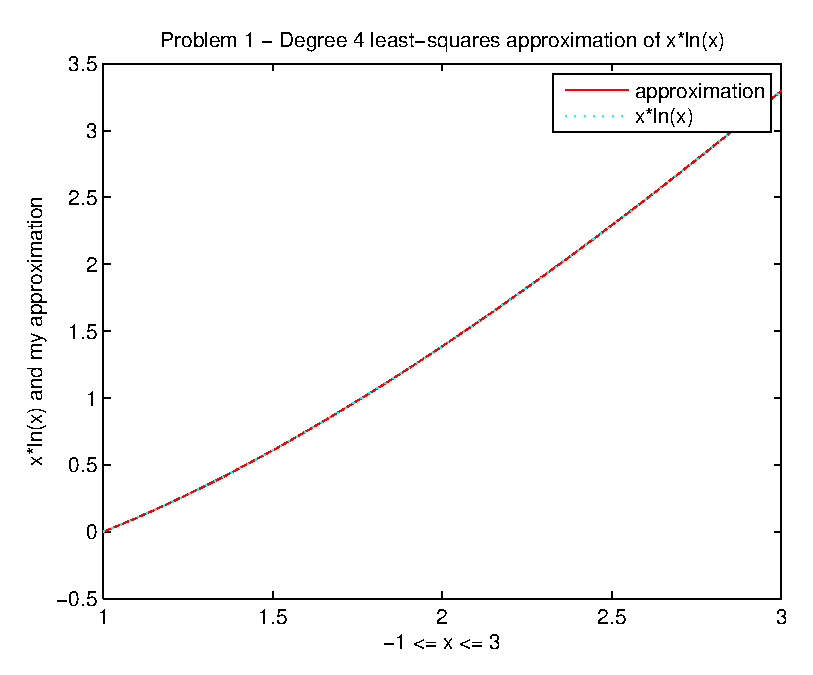
\includegraphics [width=4in]{PayneMath561Assignment2_01.eps}

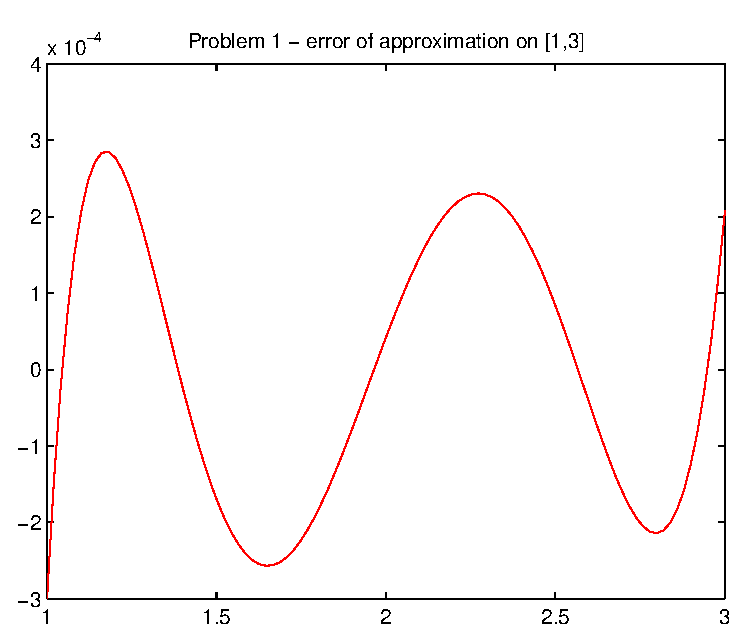
\includegraphics [width=4in]{PayneMath561Assignment2_02.eps}
\begin{verbatim}
%%%%%%%%%%%%%%%%%%%%%%%%%% PROBLEM 2 %%%%%%%%%%%%%%%%%%%%%%%%%%%%%%%%%%%%%
clear all
% Find the polynomial of degree 4 that solves the generalized interpolation
% problem: p(0) = 2, p(1) = -4,p(2) = 44, p'(0) = -9, and p'(1) = 4
% PART a) Set up and solve a system of equations
% p(x) = a4*x^4 + a3*x^3 + a2*x^2 + a1*x + a0
% p'(x) = 4*a4*x^3 + 3*a3*x^2 + 2*a2*x + a1

% Set up a matrix, A, to sovle the system
A = [1 0 0 0 0
    1 1 1 1 1
    1 2 4 8 16
    0 1 0 0 0
    0 1 2 3 4];
B = [2; -4; 44; -9; 4];

x = A\B;

% These are the coefficient values given in the output of this program
% a0 =  2
% a1 = -9
% a2 =  1
% a3 = -3
% a4 =  5

% PART b) Use a divided difference table
% xi yi/y'i
% 0    2   -9    3    7    5
% 0    2   -6    10   17
% 1   -4    4    44
% 1   -4    48
% 2    44
%
% So we have that the coefficients of the Newton Polynomial are b_i where
% b_0 = 2, b_1 = -9, b_2 = 3, b_3 = 7, b_4 = 5
%
% Then the Newton Polynomial is 2 - 9x + 3x^2 + 7x^2(x-1) + 5x^2(x-1)^2
% Using a CAS we see this simplifies to give us the 4th degree polynomial
% 5x^4 - 3x^3 + x^2 - 9x +2
% Notice that these coefficients match the results from the system of
% equations given above.
\end{verbatim}
\begin{verbatim}
%%%%%%%%%%%%%%%%%%%%%%%%%%%%%%% PROBLEM 3 %%%%%%%%%%%%%%%%%%%%%%%%%%%%%%%%
clear all
%
fs = @(x) log(x); %the function that we want to interpolate

p = @(x) log(10) *((x - 11)* (x - 12)) / 2 ...
+ log(11)* ((x - 10) *(x - 12)) / -1 + log(12)*(x - 10) *(x - 11)/2;
% p is constructed using Lagrange polynomial interpolation method

figure
fplot(fs, [10,12], 'g')
hold on
fplot(p, [10,12], '--r')
title('Problem 3 - interpolation vs. ln(x)')
legend('ln(x)', 'interpolation')
hold off

figure
fplot(fs, [11.0999 11.1001], 'g')
hold on
fplot(p, [11.0999 11.1001], 'r')
legend('ln(x)', 'interpolation')
title('Problem 3 - zoomed in at x=11.1')
% error: e_n (x) = \omega(x)/(n+1)! * f^(n+1)(\xi)
% To find the minimum and maximum bounds, we take the 3rd derivative of the
% function (since we used 3 points for interpolation) and evaluate the error
% evalute the error function at 10 and 12 for the lower and upper bounds.
syms x
f = log(x); % approximated function
f3 = diff(diff(diff(f))); % that function's 3rd derivative
poly2sym(f3, 'x');
f3 = matlabFunction(f3); % make f3 a function in matlab
omega = @(x) (x-10)*(x-11)*(x-12); % the omega function from the error formula
r = omega(11.1)/6; % evaluate omega at 11.1. 6 is (n+1)!
m = f3(10)*r; % f3*r finishes the error formula, this is the lower bound
M = f3(12)*r; % upper bound
% after running code, here are the outputs for the upper and lower bounds
%
% m =  -3.299999999999989e-05
% M =  -1.909722222222215e-05
%
\end{verbatim}

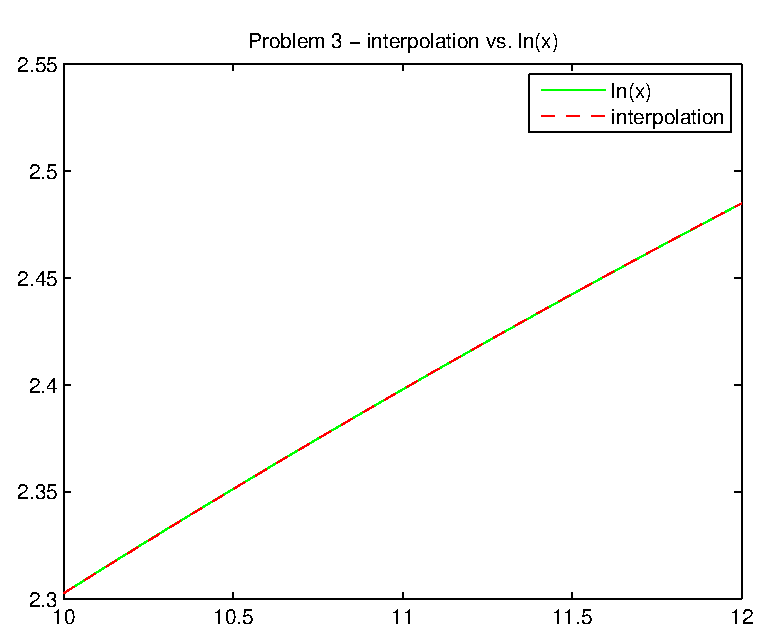
\includegraphics [width=4in]{PayneMath561Assignment2_03.eps}

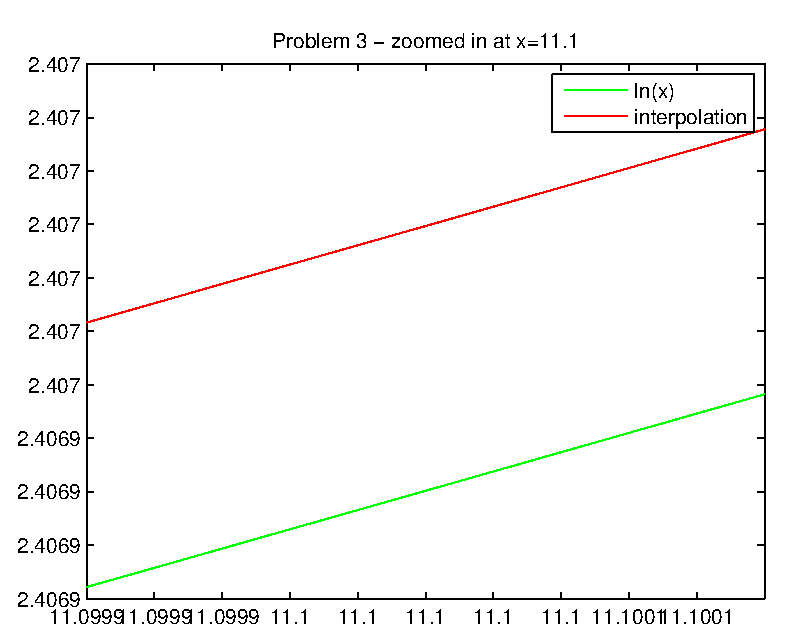
\includegraphics [width=4in]{PayneMath561Assignment2_04.eps}
\begin{verbatim}
%%%%%%%%%%%%%%%%%%%%%%%%%% PROBLEM 4 %%%%%%%%%%%%%%%%%%%%%%%%%%%%%%%%%%%%%
clear all
% The Runge Function is given by R(x) = 1/(1+25x^2)
%
% Vector containing all the points that each function will be evaluated at
e = -1:.02:1;
% PART A
% We use a matrix to find the coefficients of the interpolating polynomial
%
% Create a vector with the x-coordinates of the interpolating points
x = -1:.1:1;
%
V = vander(x);
%
% Define the runge function to get our interpolating points
R = @(x) (1+25.*x.^2).^(-1);
%
% Declare a column vector which holds the y-coordinates for our interpolating
% points
y = R(x)';
%
c = V\y;
%
% After running the code, c (a column vector with all the coefficients of
% the interpolating polynomial) is
% c = 1.0e+06 *
%
%           0.2602
%          -0.0000
%          -1.0121
%           0.0000
%           1.6392
%          -0.0000
%          -1.4429
%           0.0000
%           0.7573
%          -0.0000
%          -0.2452
%           0.0000
%           0.0493
%          -0.0000
%          -0.0061
%           0.0000
%           0.0005
%          -0.0000
%          -0.0000
%           0
%           0.0000
%
% v is the interpolating polynomial of degree 20
v = matlabFunction(poly2sym(c,'x'));
%
% PART B
%
% set xt as a vector containing the Chebyshev points
xt = cos((2.*([20:-1:0])+1).*pi./42);
% create a Vandermonde matrix
Vt = vander(xt);
yt = R(xt)';
% solves the system and sets ct as the column vector containing the
% coefficients of the interpolating polynomial at the Chebyshev points.
ct = Vt\yt;
% converts ct into an inline function to plot
vt = matlabFunction(poly2sym(ct,'x'));
%
% the coefficients of the interpolating function are:
%
%              1.0e+04 *
%
%          0.646655103655755
%         -0.000000000004668
%         -3.420805498370904
%          0.000000000021239
%          7.775445632006652
%         -0.000000000040194
%         -9.930012492409208
%          0.000000000041009
%          7.823630205987262
%         -0.000000000024462
%         -3.933329690078009
%          0.000000000008663
%          1.263561779281532
%         -0.000000000001769
%         -0.253727314541573
%          0.000000000000192
%          0.030662946960456
%         -0.000000000000009
%         -0.002176233358920
%          0.000000000000000
%          0.000100000000000
%
%
% PART C
% use spline interpolation on the 21 points from part a and evaluate the
% spline at the 101 points in vector 'e'
%
yy = spline(x, y, e);

figure
% plots each interpolation and its evaluation at the 101 points on [-1 1]
plot(e,v(e),'r', e, vt(e),'g', e,yy,'c')
ylim([-.2 1.2])
legend('interpolation', 'interpolation at cheby points', 'spline')
title('Problem 4')
\end{verbatim}

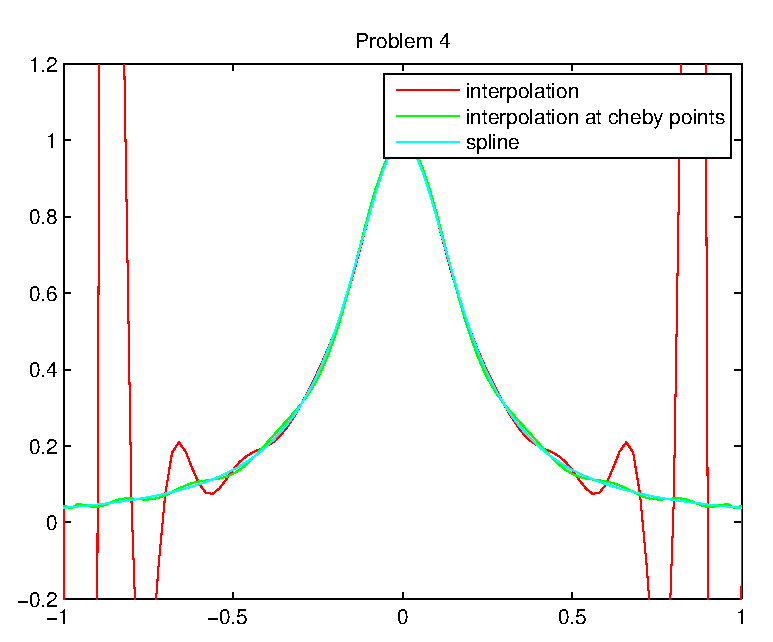
\includegraphics [width=4in]{PayneMath561Assignment2_05.eps}
\begin{verbatim}
%%%%%%%%%%%%%%%%%%%%%%%%%%%%%%% PROBLEM 5 %%%%%%%%%%%%%%%%%%%%%%%%%%%%%%%%
clear all
clc
% PART A
%
x5 = [-2 0 2 3 4 5]; % inputs
y5 = [4 0 -4 -30 -40 -50]'; % outputs of function
V = vander(x5); % declare Vandermonde matrix to find polynomial
c = V\y5; % vector with coefficients of interpolating polynomial
p = poly2sym(c, 'x');
a = -2:.1:5; % domain of the interpolation
polynomial = matlabFunction(p); % fa is the polynomial interpolation
%
% PART B
%
s = spline(x5,y5,a);
%
% PART C
%
% for clamped spline, store end conditions into new vector 'e'
e = [-2 y5' 10]';
clamped = spline(x5,e, a);
%
% PART D
%
chip = pchip(x5, y5, a);

figure
hold on
scatter(x5,y5,'o', 'c')
plot(a, polynomial(a), ':r')
plot(a, s, '--g')
plot(a, clamped, ':')
plot(a, chip, '--')
legend('data', 'polynomial', 'spline', 'clamped spline', 'pchip')
title('Problem 5')
%
\end{verbatim}

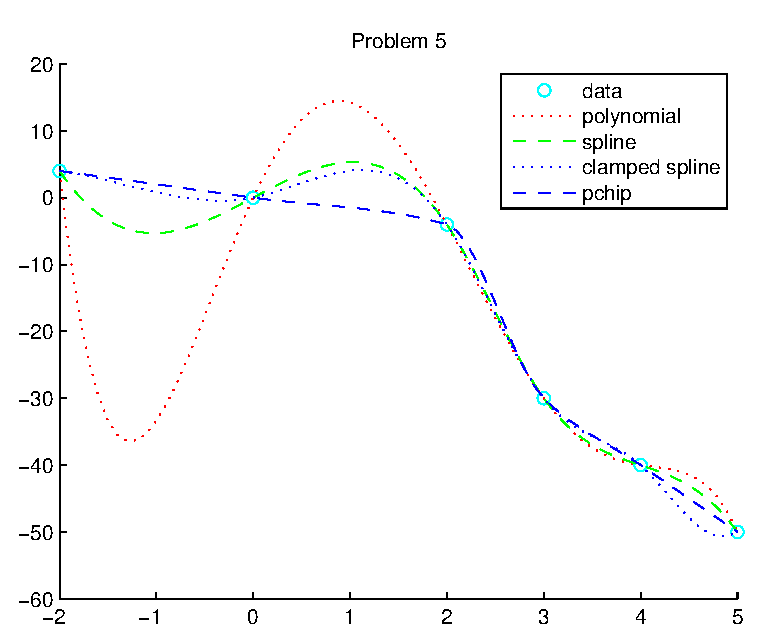
\includegraphics [width=4in]{PayneMath561Assignment2_06.eps}
\begin{verbatim}
%%%%%%%%%%%%%%%%%%%%%%%%%%% PROBLEM 6 %%%%%%%%%%%%%%%%%%%%%%%%%%%%%%%%%%%
%
\end{verbatim}
\begin{verbatim}
%%%%%%%%%%%%%%%%%%%%%%%%%%% PROBLEM 7 EXTRA CREDIT %%%%%%%%%%%%%%%%%%%%%%
%
% In MuPad, we use the Pade command to find the Pade approximation of f(x)
% = tan(x) around x=0 witn m=n=2.
% PART A
% Pade(tan(x),0,[2,2]) =
% x(x^2-15) / 3(2x^2-5)
% The Pade approximation has a singularity at x = +- sqrt(5/2)
t = [(-sqrt(5/2)) :.1: (sqrt(5/2))];
y = [-2:.1:2];
P = @(x) (x.*(x.^2-15)) ./ (3.*(2.*x.^2-5));
f = @(x) tan(x);
P1 = (y.*(y.^2-15)) / (3.*(2.*y.^2-5));
figure

plot(y, P(y), 'or')
hold on
plot(y, tan(y),'g')
ylim([-10 10])
legend('Pade', 'tangent')
title('Pade approximation at 0 with n=m=2 of tan(x)')
%
% PART B
% In MuPad, we use the Pade command to find the Pade approximation of f(x)
% = tan(x) around x=0 witn m=n=3.
%
% The Pade approximation with m=n=3 is exactly the same as m=n=2 since
% tan(x) is an odd
\end{verbatim}

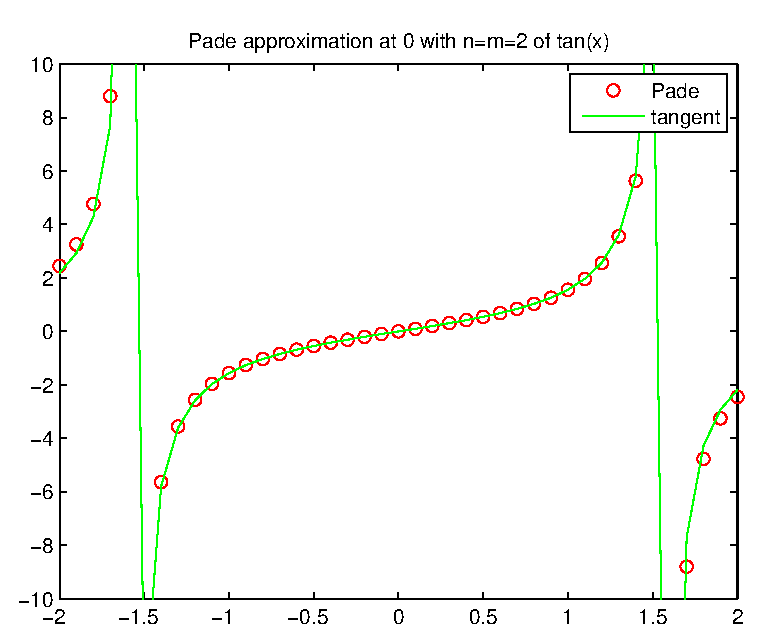
\includegraphics [width=4in]{PayneMath561Assignment2_07.eps}



\end{document}
    
